\postextualchapter{The ANN Internal Representation Space}
In this appendix, the author would like to call the attention for the interesting internal representation created by a NN. The internal representation here could be replaced by the question: "what/how do the NN neurons are firing for". The inspiration for the discussion presented here comes from the well known behavior of the Convolutional Neural Networks (CNNs). The CNNs are special because the filters created by the convolution procedure during the network training can describe objects which humans are familiar with. For instance, in face recognition the filters can (and usually do) learn properties of human face, as the noose, the eyes, the mouth and so on.

In the case of the Fully Connected NNs used in this analysis, it is not so obvious how one could extract similar features from them and in fact, there seems not to exist a work about such topic in the literature. But, motivated by how the features are extracted from the filters of a CNN, the author looked to the response coming from the neurons in different layers when the inputs are given to the NN. Then, superimposing the behavior of such neurons when responding to signal and background inputs returned some pictures like the ones showed in Fig.~\ref{fig:nn_features}. Note that, those pictures are an example since the NNs used have three layers and several neurons. Taking the NN for the \textbf{Njets2} category, for instance, it has the topology 21:15:8 and thus, (for six particles and with $p_{T}$, $\eta$, $\phi$ as inputs) it generates more than 500 pictures. Even so, it is possible to draw some observations from them and Fig.~\ref{fig:nn_features} represents well what was seen for the NN in the other neurons in each layer.

The first observation that can be quickly derived by looking through the plots in Fig.~\ref{fig:nn_features}(a), (b) and (c) is that the separation between signal (in red) and background (in blue) increases gradually across the hidden layers. This is more evident for the leptons since they do not produce discrimination between the VBF process and the other SM Higgs production modes. While that, the jets (the two highest $p_{T}$ at least) have a good separation in $\eta$ already in the first hidden layer. This is not surprising since we expect such behavior in $\eta$ for the VBF jets. It's also possible to notice that the patterns of discrimination across the hidden layers also gets more complex as the pictures changes their shapes. The most surprising observation (at the author point of view) is the separation in $\phi$, which has a exactly same distribution (roughly a uniform distribution between $-\pi$ and $+\pi$) for signal and backgrounds. Note that the plots in Fig.~\ref{fig:nn_features}(c) are not coming from the output layer, those are the responses of one of the neurons in the last hidden layer before the output neuron, which only give responses in the range [0, 1] (which are the labels for the two classes, background and VBF, respectively).

\begin{figure}[htbp]{16cm}
	\caption{The behavior of the NN neuron output for the (a) first hidden layer, (b) second hidden layer and (c) output layer. The subplots in (a), (b) and (c) show, from left to right and sorted, the $p_{T}$'s (top row), the $\eta$'s (middle row) and the $\phi$'s (bottom row) of the four leptons and the three jets.}
	\centering
	\subfloat[]{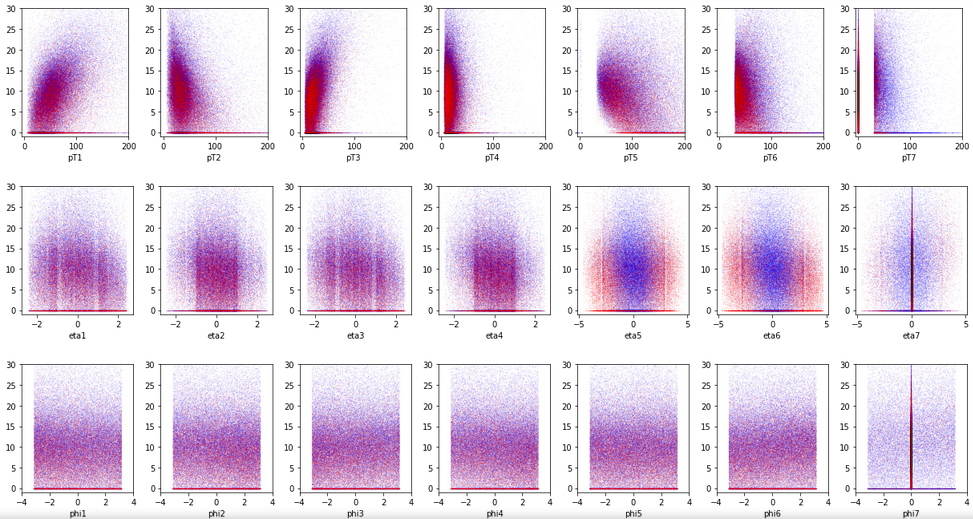
\includegraphics[scale=0.47,trim={0cm 0cm 0cm 0cm},clip]{AppendixNeuralNetwork/figs/Features/layer1_neuron0_vs_inputs}}\\
	\subfloat[]{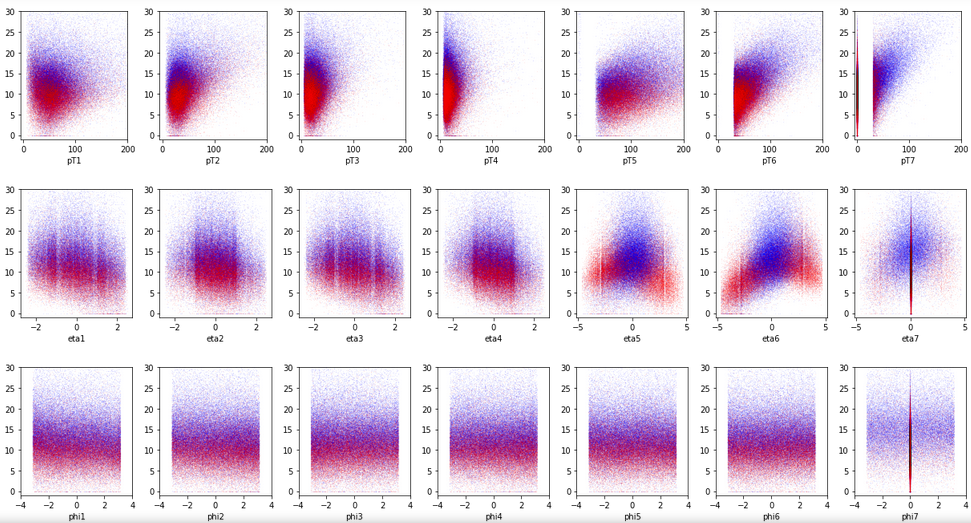
\includegraphics[scale=0.47,trim={0cm 0cm 0cm 0cm},clip]{AppendixNeuralNetwork/figs/Features/layer2_neuron4_vs_inputs}}\\
	\subfloat[]{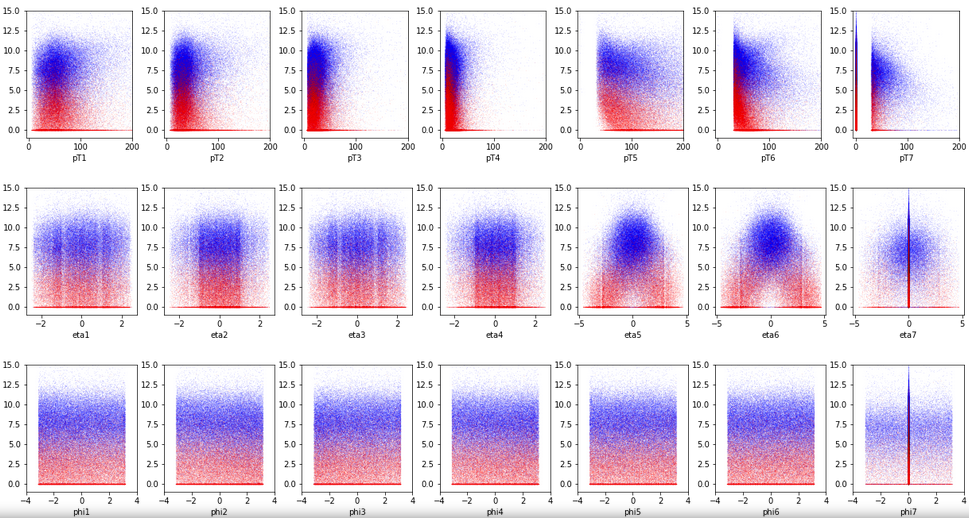
\includegraphics[scale=0.47,trim={0cm 0cm 0cm 0cm},clip]{AppendixNeuralNetwork/figs/Features/layer3_neuron1_vs_inputs}}
	\source{The author, 2018.}
	\label{fig:nn_features}
\end{figure}	